\section{Overall Architecture}
Based on the design and the the self imposed requirements the architecture has been defined which defines how all the components shall work together.
The components are described briefly as \textit{Overall Architecture} before each of the components is explained in detail in later chapters.

The overall architecture consists of the following modules
\begin{itemize}
    \item Mitosis-Core
    \item Simulation
    \item Visualisation
    \item \gls{cli}
    \item Symbiosis
\end{itemize}

The dependency graph, how all the components are wired up, is visualised in \vref{fig:mit-dependencygraph}.

\begin{figure}
\centering
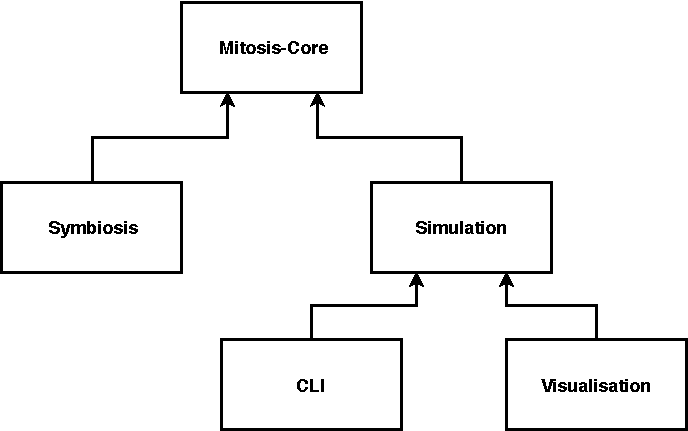
\includegraphics[width=0.75\textwidth]{graphics/implementation/overall-architecture.pdf}
\caption{Mitosis dependency graph}
\label{fig:mit-dependencygraph}
\end{figure}

\textit{Mitosis-Core} is the main component which sets up the Peer-To-Peer mesh network. The component itself handles all the logic in a transparent way, meaning that it offers a simple interface, so an application using it does not have to care about the logic behind.

The provided interface of \textit{Mitosis-Core} is used by the \textit{Simulation} component. The simulation sets up virtual peers and mocks the actual connections, so peers can exchange messages without using the physical layer. Each of the peers is initialising the \textit{Mitosis-Core} and acts like it would do in a real application

Visualising the output of the simulation, is the responsibility of the \textit{Visualisation} component. It uses the interface provided \textit{Simulation} component to paint the virtual peers with their connections. Also it provides several inspector tools to analyse for example in- or outgoing messages of each peer.

To enable bench marking with different parameters for the \textit{Mitosis-Core}, the \textit{\gls{cli}} component has been created. Similar to the Visualisation component is also uses the interface provided by the \textit{Simulation} component. However, it does not run in the browser but on a Node.js server and allows to run \textit{Mitosis-Core} with different parameters. The parameters can by provided via the command line. After a test run the \gls{cli} saves the test result as a file for further processing.

Last but not least the component \textit{Symbiosis} represents a sample use case application to demonstrate how \textit{Mitosis-Core} would be used in a real application. \textit{Symbiosis} is a video broadcasting app that allows the user to send a real-time video stream to all other peers in the network.



